\documentclass[a4paper,10pt]{article} 

\usepackage[utf8]{inputenc} 
%\usepackage[T1]{fontenc}

\usepackage{textcomp}           % Extra Symbole (Grad Celsius etc.)
\usepackage{amssymb,amsmath}    % Schöne Formeln (AMS = American Mathematical Society)
\usepackage{graphicx}           % Bilder und Seitenränder
\usepackage{subcaption}			% captions for subfigures
\usepackage{booktabs}           % Schönere Tabellen
\usepackage{colortbl}           % Farbige Tabellen

%\usepackage{tcolorbox}			% schöne bunte Boxen
\usepackage{mathtools}			% \mathclap für ordentliche \underbrace-			environments
\usepackage{geometry}			% Pagelayout mit \newgeometry, \restoregeometry
\usepackage{float}
\usepackage{wrapfig}
\usepackage{enumitem}
\usepackage{float}
\usepackage{braket}
\usepackage{caption}
\input{insbox.tex}
%\usepackage{pst-optexp}
%\usepackage{auto-pst-pdf}

\graphicspath{{./img/}}


\bibliographystyle{unsrtnat}

\renewcommand{\k}{\mathbf{k}}
\begin{document}
\begin{titlepage}
 \begin{center}
	\Large{Advanced laboratory class 2}
	\end{center}
	\begin{center}
	 \LARGE{\textbf{FP2 - Nonlinear Optics - Second Harmonic Generation}}
	\end{center}
	
	\begin{center}
	
	\large Marco \textsc{Canteri} \\
	marco.canteri@student.uibk.ac.at
	\end{center}
	
	\begin{center}
	\vspace{1cm}
	Innsbruck, \today
	\vspace{2cm}
	\end{center}
	
	\begin{center}
	\includegraphics[scale=0.4]{img/uibk} 
	\end{center}

\end{titlepage}
\begin{abstract}
In this work we generated ultraviolet light at around $317$ nm from a laser beam of $633$ nm exploiting Second Harmonic Generation (SHG), a second order non linear effect of a
potassium dihydrogen phosphate (KDP) crystal. We measured the power of the red laser as a function of the angle of a polarizer, then we studied the efficiency of the SHG with respect to the crystal angle.
\end{abstract}
\section{Introduction}
Inside a medium the relation between the polarization and the electric field $E$ is in first approximation linear. If the intensity of the electric field is strong enough, the relation between the field and the polarization is no longer linear and we can expand the relation. In general we find
\begin{equation}P_i  = \varepsilon_0\left(\sum_j \chi_{ij}^{(1)} E_j + \sum_{j,k}x_{ijk}^{(2)}E_jE_k + \sum_{j,k,l}\chi_{ijkl}^{(3)}E_jE_kE_l + \dots \right)\end{equation}
where the $\chi^{(i)}$ are tensors of rank $i+1$ and represent the $i$-order susceptibily. This leads to an entire new class of phenomen. in fact it is passible, to excite a new electric field of frequency $\omega_2$ with an electric field of frequency $\omega_1$.\\
From the Maxwell equations we can obtain \cite{saleh} the following differential equation for the electric field
\begin{equation}\left(\nabla^2 - \frac{1}{c^2}\frac{\partial^2}{\partial t^2}\right)E = \mu_0\frac{\partial^2 P_{NL}}{\partial t^2}\end{equation}
where $P_{NL}$ are the non linear terms of the polarization. We can see from this equation that the non linear polarization acts like a source for the electric field. Therefore, the electric field will oscillate at the same frequency of the polarization. Now, if we consider an exciting wave of frequency $\omega$:
\[E = \frac{1}{2}(A(\omega)e^{i\omega t} + \text{c.c.}), \]
and we neglect any non linear order greater than two, we can write $P_{NL}$ as
\[P_{NL}^i= \frac{\varepsilon_0}{4}\sum_{j,k}\chi_{jk}(A(\omega)e^{i\omega t} + \text{c.c.})^j\cdot (A(\omega)e^{i\omega t} + \text{c.c.})^k.\]
In the multiplication there are several terms, but we will focus on that which has a frequency of $2\omega$. Hence, we will look at generated light with frequency $2\omega$, this process is called Second Harmonic Generation.
\section{Experiment setup}
\begin{figure}[H]
\centering
\includegraphics[width=.5\textwidth]{setup}
%\begin{pspicture}[showgrid=false](8,2)(-3,-2)
%\pnode(1,1){A}\pnode(5,1){B}\pnode(5,-1){C}\pnode(1,-1){D}
% \optsource[position=start,innerlabel](A)(B){\parbox{1.5cm}{\centering He:Ne\\ 633\,nm}}
% \optretplate[position=0.2](A)(B){$\nicefrac{\lambda}{2}$}
% \optplate[position=0.6](A)(B){pol}
% \mirror(A)(B)(C)
% \mirror(B)(C)(D)
% \optbox[position=start,innerlabel](D)(C){PMT}
% \optbox[innerlabel,position=.5,optboxwidth=0.9](D)(C){KDP}
% \lens[position=.35,lensheight=0.6](D)(C){}
% \lens[position=.65,lensheight=0.6](D)(C){}
% \pinhole[position=.95,outerheight=.7](C)(D){}
% \drawbeam[linecolor=red]{1}{2}{3}{4}{5}{9}{7}
% \drawbeam[linecolor=blue]{7}{8}{6}
% \end{pspicture}
\caption{Experiment setup. A red laser is pumped into a KDP crystal to generate ultraviolet light at 317 nm (showed in blue in this figure) detected with a photomultiplier}\label{setup}
\end{figure}
The experiment setup is depicted in figure \ref{setup} and it consists of a Helium-Neon laser which output a light of 633 nm, followed by an half wave plate to rotate the polarization and a polarizer. Then the light is reflected with two mirrors and sent trough a potassium dihydrogen phosphate crystal. Finally the light is detected with a photomultiplier powered with 1700 V after it is collimated and filtered. \\
The crystal is mounted of rotating platform, such that it was possible to change the angle of the crystal orientation in order to study the efficiency of SHG. In fact the power of the generated light can be written as
\[I_{2\omega} \propto I_{max}\text{sinc}^2\left(L\frac{\Delta k}{2 }\right),\]
where $\Delta k = \frac{4\pi}{\lambda}(n_{2\omega} - n_\omega)$ is called the phase matching condition and $L$ is the length of the crystal. In order to get the maximum power, it must holds $\Delta k = 0$. Therefore, the refractive index at frequency $\omega$ must be equal to the refractive index of frequency $2\omega$. In a normal crystal this never occurs due to the dispersion of light, but we can exploit birefringence of the crystal. For an incident wave with angle $\theta$, the refractive index is given by the following formula \cite{saleh}
\[\frac{1}{n^2(\theta,\omega)} = \frac{\cos^2\theta}{n_o(\omega)}+\frac{\sin^2\theta}{n_e(\omega)}.\]
There are two different type of phase matching, if the incident waves have ordinary polarization it is referred as Type I phase matching, otherwise, if the waves have perpendicular polarization, it is called Type II phase matching.
\InsertBoxR{0}{
  \begin{minipage}{5.5cm}
  \includegraphics[width = 5.5cm]{elipsoid}
\end{minipage}}[3]
This condition can be visualized with the help of the so called refractive index ellipsoid. In the figure we can notice that there are some points where the extraordinary refractive index with frequency $\omega$ is equal to the ordinary refractive index with frequency $2\omega$ That is where there is phase matching.

\section{Measurements and analysis}
Before performing the measurements on SHG, we first measured the power of the laser for different angles of the polarizer. The measured were taken with a powermeter, we took 10 seconds of measurements and we used the built-in function for the average value and the standard deviation. We started from angle 0° to 360° with a step of 10 degrees. As can be seen from the plot in figure \ref{polarizer}, the data are in agreement with the theoretical law $P = P_{max}\cos^2(\theta)$, a fit has been done and it leads to $P_{max} = 7.24\pm  0.07$ mW.
\begin{figure}[H]
\centering
\includegraphics[width = \textwidth]{polarization}
\caption{Power of the Helium Neon laser as a function of the polarizer angle. The error of the angle is due to the resolution of the polarizer, anyway the error bars are to small to be seen}
\label{polarizer}
\end{figure}
Then, we set the polarizer at 180 degrees, so the light that went through the crystal was vertical polarized. Thus we measured the power of the second harmonic with a photomultiplier. We rotate the crystal along the $y$ direction. We took measure from 0° to 360° with a step of 10 degrees. In the oscilloscope we acquired data with a scale of 500 $\mu$s, we averaged these data e calculated the standard deviation in order to get an error. The plot is show in figure \ref{spectrum}
\begin{figure}[H]
\centering
\includegraphics[width = \textwidth]{spectrum}
\caption{Photomultiplier signal of the second harmonic as a function of crystal angle, experimental data are shown in point, while the line is only for eyes helping. The errors are too small and cannot be seen}
\label{spectrum}
\end{figure}

 \begin{thebibliography}{99}

  \bibitem{saleh}
  \textsc{Bahaa E. A. Saleh, Malvin Carl Teich}, \textit{Fundamentals of photonics}, Wiley series in pure and applied optics, 1991, 1st edition

  \bibitem{inequality}
   \textsc{J. F. Clauser, M. A. Horne, A. Shimony und R. A. Holt}, \textit{Proposed experiment to
test local hidden-variable theories}, Phys. Rev. Lett., 23 (1969), pp. 880–884.

\bibitem{skriptum}
Fortgeschrittenenpraktikum 2, \textit{Entanglement and Bell’s inequality}. \textsc{Gregor Weihs, Kaisa Laiho, Harishankar Jayakumar}. WS 2015/16
\end{thebibliography}
\end{document}
